\chapter{Background}
\label{cha:background}

In questo capitolo verrà descritta la piattaforma oggetto di studio, saranno inoltre
introdotte delle definizioni e concetti generali riguardanti la Threat Intelligence
e la Open Source Intelligence.

\section{SATAYO}
\label{sec:satayo}

Come accennato precedentemente, SATAYO\cite{satayo} è un servizio che colleziona,
aggrega e presenta informazioni di natura OSINT in modo semi automatico. È
disponibile in modalità \textit{One Time}, in cui un cliente può richiedere uno
scan della propria esposizione, il quale sarà consultabile per qualche settimana;
\textit{SaaS (Software as a Service)}, in cui viene continuamente monitorata l'esposizione
online di un cliente con la possibilità di consultare direttamente la
piattaforma; infine in modalità \textit{SaaS \& Managed} in cui, oltre all'accesso
diretto come in modalità SaaS, il cliente ha anche a disposizione un team di
specialisti che analizzano le evidenze collezionate e forniscono direttamente
istruzioni per eventuali mitigazioni necessarie. Le ricerche di SATAYO sono quasi
completamente automatizzate, vengono infatti svolte le azioni necessarie per il
collezionamento delle risorse senza intervento manuale: per esempio partendo da un
dominio, automaticamente vengono trovati i suoi sotto domini, che a loro volta verranno
analizzati per testare eventuali servizi esposti. Contrariamente azioni come l'inserimento
di metadati del cliente per perfezionare le ricerche, e il controllo qualità a fine
ricerca, previa pubblicazione, vengono svolte manualmente da un analista. SATAYO
non è limitato alle risorse presenti nel \textit{Surface Web}\cite{Kavallieros2021},
esegue infatti ricerche e utilizza informazioni presenti nel \textit{Deep Web}, ovvero
la parte di internet non indicizzata dai motori di ricerca, e nel \textit{Dark
Web} che è accessibile solo tramite software specifici come \texttt{Tor}\footnote{\url{https://www.torproject.org/}}.
In questa ultima porzione di internet è possibile trovare anche piattaforme in
cui vengono venduti oggetti e software illegali, come può essere l'accesso privilegiato
all'infrastruttura di un cliente.

\section{OSINT}
\label{sec:osint}

L'OSINT\cite{GLASSMAN2012673}, ovvero Open Source INTelligence, è una branca dell'intelligence
che si occupa della ricerca e analisi di dati ottenuti da fonti accessibili pubblicamente.
In generale queste informazioni possono essere ottenute da risorse di diverso
tipo, quali mezzi di comunicazione (giornali, riviste, televisione), dati
governativi pubblici, pubblicazioni accademiche, dati commerciali e, soprattutto,
dall'internet. È proprio quest'ultima la fonte principale utilizzata da SATAYO,
online infatti si trovano molte informazioni che per natura devono essere
pubbliche, ma spesso non ci si presta attenzione. Esempi di queste informazioni
possono essere: record DNS, i quali rivelano molte informazioni riguardanti il
perimetro pubblico di un'organizzazione; account su piattaforme di social network,
quali Linkedin, che riportano in modo piuttosto dettagliato la lista di dipendenti
di un'azienda con i rispettivi ruoli all'interno della stessa; market nel
\textit{Dark Web} che mettono in vendita informazioni che possono essere ritenute
pericolose se di dominio pubblico, come log rubati da macchine infette e accesso
privilegiato alla rete aziendale.

\begin{figure}[htbp]
  \centering
  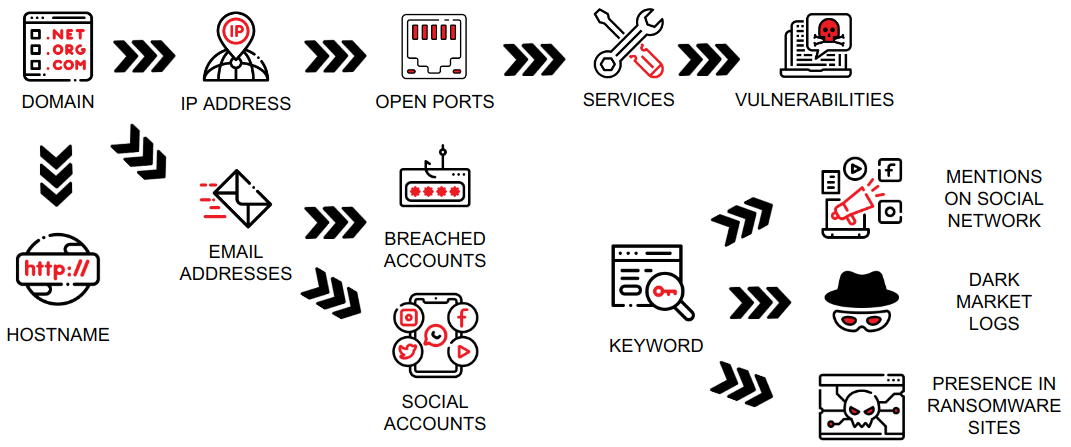
\includegraphics[width=.7\linewidth]{images/exposure_assessment.png}
  \caption{Esempio di informazioni collezionate con metodologie OSINT\cite{pavanello-master}}
  \label{fig:exposure_assessment}
\end{figure}

\pagebreak
\section{Cyber Threat Intelligence}
\label{sec:cti}

La \textit{Cyber Threat Intelligence}\cite{lee2023cyber} (CTI) rappresenta l'analisi
di intelligence ottenuta tramite fonti OSINT, file di log, analisi del traffico
di rete di un'organizzazione e analisi forensi. Lo scopo della CTI è di studiare
e individuare delle possibili minacce, sia cyber che fisiche, in modo tale da agire
proattivamente agli attacchi che si potrebbero presentare in futuro. Grazie a
questa tecnica per le aziende è possibile individuare quali minacce presentano
un rischio maggiore e agire di conseguenza. Parte della CTI è anche l'individuazione
di \textit{Threat Actors}, persone o gruppi di persone che pongono una minaccia nei
confronti di aziende e organizzazioni. Solitamente si ottengono evidenze di
questi TA tramite ricerche nel deep o dark web, vengono poi correlate le informazioni
ottenute con altri dati riguardanti i clienti per individuare eventuali minacce.